%%% Hlavní soubor. Zde se definují základní parametry a odkazuje se na ostatní části. %%%

%% Verze pro jednostranný tisk:
% Okraje: levý 40mm, pravý 25mm, horní a dolní 25mm
% (ale pozor, LaTeX si sám přidává 1in)
\documentclass[12pt,a4paper]{report}
\setlength\textwidth{145mm}
\setlength\textheight{247mm}
\setlength\oddsidemargin{15mm}
\setlength\evensidemargin{15mm}
\setlength\topmargin{0mm}
\setlength\headsep{0mm}
\setlength\headheight{0mm}
% \openright zařídí, aby následující text začínal na pravé straně knihy
\let\openright=\clearpage

%% Pokud tiskneme oboustranně:
% \documentclass[12pt,a4paper,twoside,openright]{report}
% \setlength\textwidth{145mm}
% \setlength\textheight{247mm}
% \setlength\oddsidemargin{15mm}
% \setlength\evensidemargin{0mm}
% \setlength\topmargin{0mm}
% \setlength\headsep{0mm}
% \setlength\headheight{0mm}
% \let\openright=\cleardoublepage

%% Použité kódování znaků: obvykle latin2, cp1250 nebo utf8:
\usepackage[utf8]{inputenc}

%% Ostatní balíčky
\usepackage{graphicx}
\usepackage{amsthm}
\usepackage{amssymb}
\usepackage{amsmath}
\usepackage{framed}
\usepackage[titles]{tocloft}
\usepackage[font=small,labelfont=bf]{caption}
\usepackage{chngcntr}
\counterwithout{figure}{chapter}

%% Balíček hyperref, kterým jdou vyrábět klikací odkazy v PDF,
%% ale hlavně ho používáme k uložení metadat do PDF (včetně obsahu).
%% POZOR, nezapomeňte vyplnit jméno práce a autora.
\usepackage[ps2pdf,unicode]{hyperref}   % Musí být za všemi ostatními balíčky
\hypersetup{pdftitle=Separation axioms}
\hypersetup{pdfauthor=Karel Ha}

%%% Drobné úpravy stylu

% Tato makra přesvědčují mírně ošklivým trikem LaTeX, aby hlavičky kapitol
% sázel příčetněji a nevynechával nad nimi spoustu místa. Směle ignorujte.
\makeatletter
\def\@makechapterhead#1{
  {\parindent \z@ \raggedright \normalfont
   \Huge\bfseries \thechapter. #1
   \par\nobreak
   \vskip 20\p@
}}
\def\@makeschapterhead#1{
  {\parindent \z@ \raggedright \normalfont
   \Huge\bfseries #1
   \par\nobreak
   \vskip 20\p@
}}
\makeatother

% Toto makro definuje kapitolu, která není očíslovaná, ale je uvedena v obsahu.
\def\chapwithtoc#1{
\chapter*{#1}
\addcontentsline{toc}{chapter}{#1}
}

%%%%%%%%%%%%%%%%%%%%%%%%%%%%%%%%%%%%%%%%%%%%%%
% přidal Karel Ha
\newcommand{\HRule}{\rule{\linewidth}{0.5mm}}
\theoremstyle{plain}
\newtheorem{thm}{Theorem}[section]
\newtheorem{lem}[thm]{Lemma}
\newtheorem{prop}[thm]{Proposition}
\newtheorem{cor}[thm]{Corollary}

\theoremstyle{definition}
\newtheorem*{df}{Definition}	% Definice nečíslujeme, proto "*"
\newtheorem{exmpl}{Example}
\newtheorem{fact}{Fact}
\newtheorem*{obs}{Observation}
\newtheorem*{nota}{Notation}

\theoremstyle{remark}
\newtheorem{rem}[thm]{Remark}

\numberwithin{equation}{section}
\renewcommand{\theequation}{\arabic{chapter}.\alph{equation}}

%\renewcommand{\qedsymbol}{$\boxtimes$}
\renewcommand{\qedsymbol}{$\blacksquare$}

\def\labelitemi{$\spadesuit$}
\renewcommand\thechapter{\Roman{chapter}} 
%\renewcommand\thesection{\arabic{section}}
%\renewcommand\thesubsection{(\alph{subsection})}
\renewcommand\thefigure{\Alph{figure}} 

\renewcommand{\labelenumi}{{\rm(\roman{enumi})}}

% mezera v Table of Contents před číslem kapitoly
\renewcommand*\cftchapnumwidth{2.2em}
\renewcommand*\cftsecnumwidth{2.6em}
% samotna cisla "section" misto "chapter.section"
%\renewcommand\cftchapaftersnum{}
%\renewcommand\cftsecaftersnum{.}

\newcommand{\N}{\mathbb{N}}
\newcommand{\Q}{\mathbb{Q}}
\newcommand{\I}{\mathbb{I}}
\newcommand{\Acal}{\mathcal{A}}
\newcommand{\Bcal}{\mathcal{B}}
\newcommand{\Ccal}{\mathcal{C}}
\newcommand{\D}{\mathfrak{D}}
\newcommand{\none}{\varnothing}
\newcommand{\st}{\mid}
\newcommand{\uparr}{\left\uparrow\right.}
\newcommand{\darr}{\left\downarrow\right.}
\newcommand{\dL}{\left\uparrow d_L \right.}
\newcommand{\n}{\mathfrak{n}}
\newcommand{\rb}{\prec}
\newcommand{\cb}{\prec\mkern-8mu\prec}
\newcommand{\cov}{<\mkern-12mu\cdot\mkern8mu}
\newcommand{\embed}{\buildrel\subseteq\over\longrightarrow}
\renewcommand{\phi}{\varphi}

\hyphenation{approach}
\hyphenation{ca-te-go-ry}
\hyphenation{con-ti-nuous}
\hyphenation{de-fi-ning}
\hyphenation{equi-va-len-ce}
\hyphenation{equi-va-len-ces}
\hyphenation{ge-ne-ra-ted}
\hyphenation{pro-duct}
\hyphenation{pro-ducts}
\hyphenation{se-cond-ly}
\hyphenation{se-pa-ra-tion}
\hyphenation{strong-ly}
\hyphenation{sub-lo-ca-le}
\hyphenation{to-po-lo-gy}
\hyphenation{weak-ly}
%%%%%%%%%%%%%%%%%%%%%%%%%%%%%%%%%%%%%%%%%%%%%%

\begin{document}

% Trochu volnější nastavení dělení slov, než je default.
\lefthyphenmin=2
\righthyphenmin=2

%%% Titulní strana práce

\pagestyle{empty}
\begin{center}

\large

Charles University in Prague

\medskip

Faculty of Mathematics and Physics

\vfill

{\bf\Large BACHELOR THESIS}

\vfill

\centerline{\mbox{\includegraphics[width=60mm]{../img/logo.eps}}}

\vfill
\vspace{5mm}

{\LARGE Karel Ha}

\vspace{15mm}

% Název práce přesně podle zadání
\HRule \\[0.6cm]
{\LARGE\bfseries Separation axioms} \\[0.2cm]
\HRule \\[1.5cm]

\vfill

% Název katedry nebo ústavu, kde byla práce oficiálně zadána
% (dle Organizační struktury MFF UK)
Department of Applied Mathematics

\vfill

\begin{tabular}{rl}

Supervisor of the bachelor thesis: & prof. RNDr. Aleš Pultr, DrSc. \\
\noalign{\vspace{2mm}}
Study programme: & Computer Science \\
\noalign{\vspace{2mm}}
Specialization: & General Computer Science \\
\end{tabular}

\vfill

% Zde doplňte rok
Prague 2013

\end{center}

\newpage

%%% Následuje vevázaný list -- kopie podepsaného "Zadání bakalářské práce".
%%% Toto zadání NENÍ součástí elektronické verze práce, nescanovat.

%%% Na tomto místě mohou být napsána případná poděkování (vedoucímu práce,
%%% konzultantovi, tomu, kdo zapůjčil software, literaturu apod.)

\openright

\noindent
\section*{Acknowledgement}

I wish to express my deepest gratitude to my advisor, professor Aleš Pultr, for
his helpful suggestions, constructive criticism, excellent tutoring and, above
all, for showing me how ``pointless'' topology can be.

I would also like to thank my loving and caring family, whose support in (not
only) the most desperate times of my studies will always be appreciated.

My further thanks belong to my dear friend Filip Miller for all his fruitful
comments concerning English language.

Last but not least, I would like to pay tribute to my patient mentors at~the
Charles University in~Prague for guiding me through the thorny path of~academic
life and enabling me to truly develop as a~person.

\newpage

%%% Strana s čestným prohlášením k bakalářské práci

\vglue 0pt plus 1fill

\noindent
I declare that I carried out this bachelor thesis independently, and only with the cited
sources, literature and other professional sources.

\medskip\noindent
I understand that my work relates to the rights and obligations under the Act No.
121/2000 Coll., the Copyright Act, as amended, in particular the fact that the Charles
University in Prague has the right to conclude a license agreement on the use of this
work as a school work pursuant to Section 60 paragraph 1 of the Copyright Act.

\vspace{10mm}

\hbox{\hbox to 0.5\hsize{%
In Prague, May 22, 2013
\hss}\hbox to 0.5\hsize{%
Karel Ha
\hss}}

\vspace{20mm}
\newpage

%%% Povinná informační strana bakalářské práce

\vbox to 0.5\vsize{
\setlength\parindent{0mm}
\setlength\parskip{5mm}

Název práce:
Oddělovací axiomy
% přesně dle zadání

Autor:
Karel Ha

Katedra:  % Případně Ústav:
Katedra aplikované matematiky
% dle Organizační struktury MFF UK

Vedoucí bakalářské práce:
prof. RNDr. Aleš Pultr, DrSc., Katedra aplikované matematiky
% dle Organizační struktury MFF UK, případně plný název pracoviště mimo MFF UK

Abstrakt:
% abstrakt v rozsahu 80-200 slov; nejedná se však o opis zadání bakalářské práce
Klasická (bodová) topologie se zabývá body a~vztahy mezi nimi a~ur\-či\-tý\-mi
podmnožinami.
Když odhlédneme od bodů a uvážíme pouze strukturu o\-te\-vře\-ných množin,
získáme tzv. \emph{frame\/} neboli úplný svaz splňující distributivní zákon $b
\wedge \bigvee A = \bigvee \{ b \wedge a \st a\in A \}$.
Ten je důležitým konceptem bezbodové topologie.

Bezbodový přístup (při téměř nepatrné ztrátě informací) nám poskytuje hlubší
poznatky o~topologii.
Příkladem je studium oddělovacích axiomů.
Tato práce je zaměřena na $T_i$-axiomy (pro $i = 0, 1, 2, 3, 3\frac{1}{2}, 4$),
tj. vlastnosti topologických prostorů zahrnující oddělování bodů od sebe,
oddělování bodů od uzavřených množin a~oddělování uzavřených množin samotných.
V~této práci probereme jejich bezbodové protějšky a~způsoby, kterými na~sobě
závisí.

Klíčová slova:
% 3 až 5 klíčových slov
bezbodová topologie, oddělovací axiomy, locale, frame

\vss}\nobreak\vbox to 0.49\vsize{
\setlength\parindent{0mm}
\setlength\parskip{5mm}

Title:
% přesný překlad názvu práce v angličtině
Separation axioms

Author:
Karel Ha

Department:
Department of Applied Mathematics
% dle Organizační struktury MFF UK v angličtině

Supervisor:
prof. RNDr. Aleš Pultr, DrSc., Department of Applied Mathematics
% dle Organizační struktury MFF UK, případně plný název pracoviště
% mimo MFF UK v angličtině

Abstract:
% abstrakt v rozsahu 80-200 slov v angličtině; nejedná se však o překlad
% zadání bakalářské práce
The classical (point-set) topology concerns points and relationships between
points and subsets.
Omitting points and considering only the structure of~open sets leads to~the
notion of~\emph{frames\/}, that is, a~complete lattice satisfying the
distributive law $b \wedge \bigvee A = \bigvee \{ b \wedge a \st a\in A \}$,
the crucial concept of~point-free topology.

This pointless approach---while losing hardly any information---provides us
with deeper insights on topology.
One such example is the study of~separation axioms.
This thesis focuses on~the $T_i$-axioms (for $i = 0, 1, 2, 3, 3\frac{1}{2},
4$):
properties of~topological spaces which regard the separation of~points, points
from closed sets, and closed sets from one another.
In~this text we discuss their point-free counterparts and how they
relate to~each other.

Keywords:
% 3 až 5 klíčových slov v angličtině
pointless topology, point-free topology, separation axioms, locale, frame

\vss}

\newpage

%%% Strana s automaticky generovaným obsahem bakalářské práce. U matematických
%%% prací je přípustné, aby seznam tabulek a zkratek, existují-li, byl umístěn
%%% na začátku práce, místo na jejím konci.

\openright
\pagestyle{plain}
\setcounter{page}{1}
\tableofcontents

%%% Jednotlivé kapitoly práce jsou pro přehlednost uloženy v samostatných souborech
\chapter*{Introduction}
\addcontentsline{toc}{chapter}{Introduction}

In classical topology, spaces are often specified by \emph{separation axioms\/}
of~various strength.
The stronger axiom we have, the more ``geometrical'' a~space appears to be.

The best-known of~them are the~$T_i$-axioms ($i = 0, 1, 2, 3, 3\frac{1}{2},
4$).
They concern the separation of~points, points from closed sets, and closed sets
from each other.
The role of~points seems to be fundamental, and therefore, it may seem hard to
find natural counterparts of the $T$-axioms in the point-free context.
Nevertheless, most of them do have pointless equivalents.
The aim of this thesis is to provide their summary and to show their mutual
relationships.

\section*{Structure of thesis}

The first chapter contains the necessary concepts of~order and category
theories, followed by the essentials of~point-set and point-free topology.

In the subsequent chapter we discuss the \emph{subfitness\/}---a~weakened form
of~the $T_1$-axiom (the $T_1$-axiom itself does not seem to have a~very natural
counterpart).
It should be noted that the subfitness is crucial for some relationships
between other axioms.
Besides, it makes good sense in~classical topology as well, and moreover, plays
a~role in~logic.

The \emph{Hausdorff\/} axiom ($T_2$) does not have a~unique direct counterpart.
Unlike in~the other cases, one has several non-equivalent alternatives.
The two most standard ones are discussed in chapter III and in chapter IV we
present a~survey of~several others.

Chapters V and VI are devoted to the \emph{regularity\/} and \emph{complete
regularity\/}.
We show how to exclude points from their definitions via ``rather-below''
relation $\rb$ and ``completely-below'' relation $\cb$, and thus, how to create
their point-free analogies.

The final chapter concerns \emph{normality\/}, the translation of~which is
perhaps the easiest one.
We discuss the relation with the other axioms.

\chapter*{Preliminaries}
\addcontentsline{toc}{chapter}{Preliminaries}

\section*{Notations}

\begin{itemize}
\item $A \Subset B$ means {\sl set $A$ is a finite subset of set $B$\/}.
\item $\overline{S}$ 
\item $\Omega(X)$ denotes the lattice (or more specifically, the frame) of open
sets in $X$ together with $\subseteq$ as the ordering. 
By an abuse of notation, we denote the related underlying set in the very same
way.
\end{itemize}

\section*{Definitions}

\subsection*{Point-set topology}

Some basic notions and facts about classical topology:

\begin{itemize}
\item A \emph{topological space} is a
\item A \emph{basis} of a topological space is a
\item Likewise, a \emph{subbasis} of a topological space is a
\end{itemize}

\begin{fact}
  The topological space $\left( \prod_{i\in J} X_i, \mathcal{S} \right)$, where
  $\mathcal{S} = \left\{ p_{i}^{-1}[U] \st i\in J, \; U\in \tau_i \right\}$
  denotes its subbasis, is the product of topological spaces $\left( X_i
  \right)_{i\in J}$;
  more precisely, the projections $\left( p_i: \left(\prod_{i\in J} X_i,
  \mathcal{S}\right) \to \left(X_i, \tau_i\right) \right)_{i\in J}$
  constitute the product in~the~category~{\bf Top}.
\end{fact}

\subsection*{Point-free topology}

\begin{itemize}
\item A \emph{frame} is a
\end{itemize}

\subsection*{Category theory}

\begin{itemize}
\item A \emph{category} is a
\item A \emph{product} of a system $\left(A_i\right)_{i\in J}$ is a
\end{itemize}

\section*{Convention}

In the whole text we will omit the $T_0$ axiom, that is, we will assume all
topological spaces to be $T_0$-spaces.
Specifically, every topological space $(X, \tau)$ is considered to always
satisfy the condition
\begin{center} \it
  for any $x \ne y$ from $X$ there is an open set $U \in \tau$ such that $x \in U
  \not\owns y$ or $y \in U \not\owns x$.
\end{center}

\chapter{Weak and strong Hausdorff}

In this chapter we will contemplate point-free analogies of the $T_2$
axiom---a~separation slightly intricate to imitate in frames.
Rather, two resembling conditions will be presented.

\section{The $T_2$ axiom}

\begin{framed}
  \begin{df}[$T_2$]
    A topological space $(X, \tau)$ is called \emph{Hausdorff\/} (or, as well,
    the~\emph{$T_2$-space\/}) whenever
    \begin{center} \it
      for any $x \ne y$ from~$X$ there are open $U\owns x$ and $V\owns y$
      disjoint from~each other.
    \end{center}
  \end{df}
\end{framed}

\begin{rem} \label{T2->T1}
  Trivially from the definitions every $T_2$-space is, additionally, $T_1$.
  Thus, the sets of the form $X\setminus \left\{x\right\}$ are among the
  elements of $\Omega(X)$ (viz \ref{T1Char}).
\end{rem}

\section{The Dowker-Strauss approach}

In 1972 Dowker and Strauss \cite{ds72} introduced the condition:

\begin{framed}
  \begin{df}[$S_2'$]
    A locale $L$ satisfies the $S_2'$ axiom if for any $a, b \ne 1$ we have
    \[
      a \vee b = 1 \qquad \Rightarrow \qquad \exists u\not\leq a, v\not\leq
      b: \quad u \wedge v = 0.
    \]
  \end{df}
\end{framed}

As we are about to comprehend, it suitably ``mimics'' the Hausdorff property.

\begin{prop} \label{S2'->Haus}
  For $S_2'$-locale $\Omega(X)$ the corresponding space $X$ is always
  Hausdorff.
\end{prop}

\begin{proof}
  Recall~\ref{T2->T1}.
  Having open sets $a := X \setminus \left\{x\right\}$ and $b := X \setminus
  \left\{y\right\}$ with evident $a \cup b = X$, we acquire the $u$, $v$ from
  the $(S_2')$ definition.
  Since $u\not\subseteq X\setminus \left\{x\right\}$, the element $x$ has to
  belong to $u$.
  By symmetry, also $y \in v$.
\end{proof}

For our purposes, nevertheless, $S_2'$ will be replaced by a~somewhat weaker
description:

\begin{framed}
  \begin{df}[DS-Haus]
    A locale $L$ is considered to be \emph{weakly Hausdorff\/} (also
    \emph{DS-Hausdorff} as in \emph{Dowker-Straus-Hausdorff}) if
    \[
      a \vee b \not\in \left\{a, b\right\} \qquad \Rightarrow \qquad \exists
      u\not\leq a, v\not\leq b: \quad u \wedge v = 0.
    \]
  \end{df}
\end{framed}

\begin{rem}
  The analogous observation as in~Proposition~\ref{S2'->Haus} holds:
  because
  \[
    (X \setminus \left\{x\right\}) \cup (X \setminus \left\{y\right\}) = X
    \not\in \left\{X \setminus \left\{x\right\}, X \setminus \left\{y\right\}
    \right\},
  \]
  for the rest of the proof we can easily proceed in the same way.
\end{rem}

\section{Isbell's adaptation}

\chapter{Weakly and strongly Hausdorff}

In this chapter we will consider two point-free analogies of the $T_2$ axiom:
a~separation not quite easy to imitate in frames.

\section{The $T_2$ axiom}

\begin{framed}
  \begin{df}[$T_2$]
    A topological space $(X, \tau)$ is called \emph{Hausdorff\/} (also equally
    a~\emph{$T_2$-space\/}) if
    \begin{center} \it
      for any $x \ne y$ from~$X$ there are disjoint $U$ and $V$ with $U\owns x$
      and $V\owns y$.
    \end{center}
  \end{df}
\end{framed}

\begin{figure}[h]
  \centering
  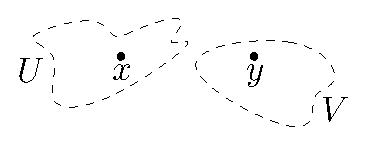
\includegraphics[height=13mm]{../img/t2.eps}
  \caption{$T_2$ property}
\end{figure}

\begin{rem} \label{T2->T1}
  Trivially, every $T_2$-space is $T_1$.
\end{rem}

\section{The Dowker-Strauss approach}

In 1972 Dowker and Strauss \cite{ds72} introduced the following condition:

\begin{framed}
  \begin{df}
    A locale $L$ satisfies the $S_2'$ axiom if
    \[
      (S_2') \qquad
      a, b \ne 1 \text{ and } a \vee b = 1 \quad \Rightarrow \quad \exists
      u\not\leq a, v\not\leq b, \quad u \wedge v = 0.
    \]
  \end{df}
\end{framed}

Its relationship to the Hausdorff property is seen from following
\begin{thm} \label{thm:T2=S2'+Sfit}
  For the $\Omega(X)$ of any topological space $X$ we have
  \[
    (T_2) \; \equiv \; (S_2') \& (\text{Sfit}).
  \]
\end{thm}

\begin{lem} \label{Haus->S2'}
  The $\Omega(X)$ of a~Hausdorff $X$ satisfies $S_2'$.
\end{lem}
\begin{proof}
  Open sets $A, B \ne X$ with $A \cup B = X$ contain some $x\in X\setminus A =
  B\setminus A$ and some $y\in X\setminus B = A\setminus B$.
  Particularly, we observe $x \ne y$ and, on top of that, receive the disjoint
  $U$ and $V$ from $(T_2)$.
  Also, $U\not\subseteq A$ (because of $x$) and $V\not\subseteq B$ (because of
  $y$).
\end{proof}

\begin{lem} \label{lem:S2'+Sfit->T1}
  $(S_2') \& (\text{Sfit}) \, \Rightarrow \, (T_1)$.
\end{lem}
\begin{proof}
  Using Fact~\ref{T1Char} on page~\pageref{T1Char}, we will show that $\{ x \}
  = \overline{\{ x \}}$.

  Assume, for the sake of contradiction, that there is $z\in \overline{\{ x \}}
  \setminus \{ x \}$.
  Since we still suppose $(T_0)$, we have $x\not\in \overline{\{ z \}}$.
  Recall Proposition~\ref{Sfit-char} on~page~\pageref{Sfit-char} and consider
  $y\in \overline{\{x\}}$ with $\overline{\{y\}} \subseteq X\setminus
  \overline{\{ z \}}$, i. e., $\overline{\{ y \}} \cap \overline{\{ z \}} =
  \none$.

  For open $A := X \setminus \overline{\{ y \}}$ and $B := X \setminus
  \overline{\{ z \}}$ we have $A \cup B = X$, and hence, also the $U, V$
  from~$(S_2')$.
  Thus, there must be $y'\in \overline{\{ y \}} \cap U$, and consequently,
  $y\in U$ (else $y'\in U\not\owns y$ would lead to $y'\not\in \overline{\{ y
  \}}$).
  Likewise, $z\in V$.
  However, $U$ and $V$ cannot be disjoint:
  as $y\in \overline{\{ x \}}$ resp. $z\in \overline{\{ x \}}$ implies $x\in U$
  resp. $x\in V$.
\end{proof}

\begin{lem} \label{lem:S2'+T1->T2}
  $(S_2') \& (T_1) \, \Rightarrow \, (T_2)$.
\end{lem}
\begin{proof}
  For open $A := X\setminus \{ x \}$ and $B := X\setminus \{ y \}$ take the
  disjoint $U, V\in \Omega(X)$ from $(S_2')$.
  Thus, $U\not\subseteq A$ resp. $V\not\subseteq B$ translates to $U\owns x$
  resp. $V\owns y$.
\end{proof}

\begin{proof}[Proof of~{\bf\ref{thm:T2=S2'+Sfit}}]
  ~

  $\Rightarrow$:
  By~\ref{T2->T1} and \ref{T1->Sfit} (on page~\pageref{T1->Sfit}), we get the
  subfitness, and using~\ref{Haus->S2'}, also the axiom $(S_2')$.

  $\Leftarrow$:
  Apply lemmata \ref{lem:S2'+Sfit->T1} and \ref{lem:S2'+T1->T2}.
\end{proof}

The $(S_2')$ axiom is often replaced by a~somewhat stronger condition:

\begin{framed}
  \begin{df}[DS-Haus]
    A locale $L$ is said to be \emph{weakly Hausdorff\/} (also
    \emph{DS-Hausdorff} as in \emph{Dowker-Straus-Hausdorff}) if
    \[
      a \vee b \not\in \left\{a, b\right\} \qquad \Rightarrow \qquad \exists
      u\not\leq a, v\not\leq b, \quad u \wedge v = 0.
    \]
  \end{df}
\end{framed}

\begin{prop} \label{prop:DS-Haus->S2'}
  (DS-Haus) implies $(S_2')$.
\end{prop}
\begin{proof}
  If $a \vee b = 1$ and $a, b \ne 1$ then $a \vee b\not\in \{ a, b \}$.
\end{proof}

\section{Isbell's approach}

Here is a~characterization of~the classical~$T_2$:

\begin{prop}
  A topological space $X$ is Hausdorff space if and only if the~diagonal
  $\Delta = \left\{(x, x) \st x\in X \right\}$ is closed in the product
  $X\times X$.
\end{prop}

\begin{proof}
  $\Rightarrow:$ Any element $(x, y)\not\in \Delta$, that means $x \ne y$, is
  separable from $\Delta$:
  namely, by~the~open $p_1^{-1}[U] \cap p_2^{-1}[V]$ with non-intersecting $U$
  and $V$ from the definition of~$(T_2)$.
  Hence, $(x, y)\not\in \overline{\Delta}$ concludes to $\Delta =
  \overline{\Delta}$, which is closed.

  $\Leftarrow:$ Choose $x \ne y$, in other words, $(x, y)\not\in \Delta$.
  Then $(x, y)$ has an open basic neighbourhood $U_1\times U_2$ disjoint from
  $\Delta$.
  That is, $U_1 \cap U_2 = \none$.
\end{proof}

This was used by Isbell \cite{isbell72} for the point-free counterpart of the
$T_2$ axiom:
Hausdorff locales are defined as those in which the~codiagonal (see
page~\pageref{codiag-in-Frm})
\[
  \nabla\colon L \oplus L \to L
\]
is a closed sublocale (see page~\pageref{df:closed-sloc}).
Since $\nabla(U) \le 0 \, \equiv \, U \subseteq \Delta(0)$, the closure of~the
codiagonal (recall \ref{prop:sloc-closure}) is $\check{d_L} = (U
\mapsto U \vee d_L)$ where
\[
  d_L
  = \bigvee \{ U \st \nabla(U) = 0 \}
  = \bigvee \{ U \st U \subseteq \Delta(0) \}
  = \Delta(0).
\]
Following from Corollary~\ref{cor:closed-sloc}, the condition proposed by
Isbell reduces~to

\begin{framed}
  \begin{df}[I-Haus]
    A locale $L$ is \emph{strongly Hausdorff\/} (or \emph{I-Hausdorff}: short
    for \emph{Isbell-Hausdorff}) if there is a~mapping $\alpha\colon L \to
    \dL$ such that
    \[
      \alpha \nabla = (U \mapsto U \vee d_L).
    \]
  \end{df}
\end{framed}

Note that the isomorphism~$\alpha$ has to be the restriction of~$\Delta$ to $L
\to \dL$.
We~have $\alpha^{-1} \check{d_L} = \nabla$, and hence,
\[
\Delta
= \nabla_*
= (\alpha^{-1} \check{d_L})_*
= (\check{d_L})_* \alpha
= j \alpha
\]
because the embedding $j\colon \dL \embed L \oplus L$ is the right adjoint
to~$\check{d_L}$ (see \ref{lem:embed-adjoint}).

\begin{lem} \label{lem:IHaus->dL}
  In an~I-Hausdorff locale~$L$ it holds that $\Delta[L] = \dL$.
\end{lem}
\begin{proof}
  As $\alpha$ is the restriction of~$\Delta$ and also an~isomorphism, we get
  $\Delta[L] = \alpha[L] = \dL$.
\end{proof}

\begin{thm} \label{IHaus->DSHaus}
  (I-Haus) implies (DS-Haus).
\end{thm}

\begin{lem} \label{lem:delta-nabla=id}
  In case of a strongly Hausdorff locale $L$, we have
  \[
    \Delta\nabla(U) = U
  \]
  for any saturated $U \supseteq d_L$.
\end{lem}
\begin{proof}
  By Lemma~\ref{lem:IHaus->dL}, every saturated $U\in \dL = \Delta[L]$ is an
  image $\Delta(a)$ for some $a\in L$.
  Let us write $\delta(U)$ for this $a$.
  In other words, $\Delta\delta(U) = U$.

  The frame codiagonal is an epimorphism and hence---as~we have $\nabla \Delta
  \nabla = \nabla$ by Fact~\ref{lrl=l} on page~\pageref{lrl=l}---we also get
  $\nabla \Delta = id$.

  Joining these two observations:
  \[
    \nabla (U) = \nabla (\Delta\delta (U)) = (\nabla \Delta)\delta (U) =
    \delta(U),
  \]
  which produces the desired $U = \Delta \delta (U) = \Delta \nabla (U)$.
\end{proof}

\begin{prop} \label{meets-in-satur}
  A~locale~$L$ is I-Hausdorff iff one has the~implication
  \begin{equation} \label{eq:meets-in-satur}
    \left( a \wedge b, a \wedge b \right) \in U
    \; \Rightarrow \;
    \left( a, b \right) \in U
  \end{equation}
  for all saturated $U \supseteq d_L$.
\end{prop}
\begin{proof}
  $\Rightarrow$:
  Whenever $(a \wedge b, a \wedge b)\in U$, we see from the formula for
  $\nabla$ that
  \[
    a \wedge b \leq \bigvee \left\{ x \st (x, x) \in U \right\} = \nabla(U).
  \]
  Having in mind the formula for $\Delta$, immediately $(a, b) \in \Delta(
  \nabla(U) ) = U$
  (the final equality by Lemma~\ref{lem:delta-nabla=id}).

  $\Leftarrow$:
  Let the condition hold and~let $a_i\in L$ for $i\in J$. 
  Since for any~saturated down-set~$U \supseteq d_L$ we have $(a_i, a_i) \in U
  \Rightarrow (a_i \wedge a_j, a_i \wedge a_j) \in U$, we also obtain
  the~implication
  \begin{equation} \label{eq:IHaus-impl}
    (a_i, a_i) \in U \Longrightarrow \{ (a_i, a_j) \st j\in J \} \subseteq U
    %\tag{\arabic{chapter}.\thesection}
  \end{equation}

  We will prove that $\alpha := (a \mapsto (a \oplus a) \vee d_L)$ satisfies
  the definition.
  Using
  \[
    \bigvee_{i\in J} a_i \oplus \bigvee_{j\in J} a_j
    = \iota_1 \left( \bigvee_{i\in J} a_i \right) \wedge \iota_2 \left(
    \bigvee_{j\in J} a_j \right)
    = \bigvee_{i, j\in J} \left( \iota_1(a_i) \wedge \iota_2(a_j) \right)
    = \bigvee_{i, j\in J} \left( a_i \oplus a_j \right)
  \]
  (the latter equality by double application of frame distributivity), we see
  that $\alpha$~preserves suprema:
  \begin{align*}
    \alpha \left( \bigvee_{i\in J} a_i \right)
    &= \left(\bigvee_{i, j\in J} \left( a_i \oplus a_j \right)\right) \vee d_L
    = \bigvee_{i\in J} \left(\left( a_i \oplus a_i \right) \vee d_L \right)
    = \bigvee_{i\in J} \alpha \left( a_i \right)
  \end{align*}
  (by~\eqref{eq:IHaus-impl} the second and the third expressions have identical
  upper bounds).
  Thus, both $\alpha$ and $\nabla$ preserve joins and~so does $\alpha \nabla$. 

  Furthermore, we have
  \[
    \alpha \nabla (a \oplus b)
    = \alpha (a \wedge b)
    = ((a \wedge b) \oplus (a \wedge b)) \vee d_L
    = (a \oplus b) \vee d_L,
  \]
  the last equality stipulated by assumed implication
  \eqref{eq:meets-in-satur}.

  In~conclusion,
  \begin{flalign*}
    \alpha \nabla (U)
    &= \alpha \nabla \left(\bigvee \{a \oplus b \st (a, b)\in U\}\right)
    = \bigvee \{\alpha \nabla \left(a \oplus b \right) \st (a, b)\in U\} \\
    &= \bigvee \{a \oplus b \vee d_L \st (a, b)\in U\}
    = \bigvee \{a \oplus b \st (a, b)\in U\} \vee d_L
    = U \vee d_L,
  \end{flalign*}
  as the elements $a \oplus b$ generate $L \oplus L$ (see
  page~\pageref{a+b-gen}).
\end{proof}

\begin{lem} \label{downsets-satur}
  The down-set
  \[
    U = \left\downarrow(a, a \wedge b)\right. \cup \left\downarrow(a \wedge b,
        b)\right. \cup \n
  \]
  is saturated in $L \times L$ for arbitrary $a, b\in L$.
\end{lem}
\begin{proof}
  Recall the saturatedness on~page~\pageref{df:satur}.
  First of all, let us have $(x_i, y)\in U$ for $i\in J$.

  \underline{Case $y = 0$}:
  obviously, $(\bigvee_{i\in J} x_i, y) = (\bigvee_{i\in J} x_i, 0)\in \n$.

  \underline{Case $y \ne 0$ and $y \leq a \wedge b$}:
  then it must be that $x_i \leq a$ in~any case.
  Thus, $(\bigvee_{i\in J} x_i, y) \in \left\downarrow(a, a \wedge b).\right.$

  \underline{Case $y \ne 0$ and $y \not\leq a \wedge b$}:
  we have both $y \leq b$ and $x_i \leq a \wedge b$.
  Hence, again $(\bigvee_{i\in J} x_i, y) \in \left\downarrow(a \wedge b,
  b)\right. \subseteq U$.

  The $(x, \bigvee_{i\in J} y_i)$ by symmetry.
\end{proof}

\phantomsection
\label{sec:overline S2}
Now we can prove the theorem.
In fact, we are going to imply a~stronger version of the (DS-Haus):
\[
  a \vee b \not\in \left\{a, b\right\} \qquad \Rightarrow \qquad \exists
  u\not\leq b, v\not\leq a: \quad u \wedge v = 0, \quad \boxed{\left(u,
  v\right) \leq \left(a, b\right)}
\]

\begin{proof}[Proof of~{\bf \ref{IHaus->DSHaus}}]
  For a contradiction: let there be an I-Hausdorff $L$, which is not weakly
  Hausdorff.
  That means, we have $a, b$ with $a \not\leq b, \, b \not\leq a$ and such that
  \[
    u \wedge v = 0 \quad \& \quad \left(u, v\right) \leq \left(a, b\right)
    \qquad \Longrightarrow \qquad
    u \leq b \; \textrm{ or } \; v \leq a.
  \]
  Especially, for the down-set $U$ taken from~\ref{downsets-satur} we have
  \begin{equation} \label{eq:dl-aoplusb}
    d_L \cap (a \oplus b) \subseteq U.
  \end{equation}

  Following from~\ref{meets-in-satur}, the saturated $(\left(a \wedge b\right)
  \oplus \left(a \wedge b\right)) \vee d_L \supseteq d_L$ contains $(a, b)$
  as it trivially contains $\left( a \wedge b, a \wedge b \right)$.
  Hence,
  \begin{align*}
    (a, b) &\in (a \oplus b) \; \cap \; (((a \wedge b) \oplus (a \wedge b))
            \vee d_L) \\
           &= ((a \wedge b) \oplus (a \wedge b)) \; \vee \; ((a \oplus b) \cap
               d_L) \\
           &\subseteq ((a \wedge b) \oplus (a \wedge b)) \; \vee \; U \\
           &= U.
  \end{align*}
  The first equality using~distributivity and the fact that $(a \wedge b)
  \oplus (a \wedge b) \subseteq a \oplus b$;
  the inclusion by~(\ref{eq:dl-aoplusb});
  the final equality from $(a \wedge b) \oplus (a \wedge b) \subseteq U$.

  This leads to the contradiction:
  $(a, b)\not\in \n$ since neither $a$ nor $b$ may equal $0$ (by $a \not\leq b,
  \, b \not\leq a$).
  Thus, the only options available are either $a \leq a \wedge b$ or $b \leq a
  \wedge b$.
  However, those stipulate $a \leq b$ or $b \leq a$ respectively,
  a~contradiction. 
\end{proof}

\chapter{More Hausdorff type axioms}

There are other $(T_2)$-type axioms for frames.
The aim of this chapter is to give a confrontation of the Dowker-Strauss
definition with axioms proposed by other pointless topologists.

\section{Variants of (DS-Haus)}

\subsection{The axiom of Johnstone and Sun Shu-Hao}

Johnstone and Sun Shu-Hao \cite{johnstone-shu-hao} suggest the axiom
\[
  (T_2') \qquad
  1 \ne a\not\le b \quad \Rightarrow \quad \exists u\not\leq a, v\not\leq b,
  \quad u \wedge v = 0.
\]
Let us also introduce its weaker version
\[
  (S_<) \qquad
  1 \ne a > b \quad \Rightarrow \quad \exists u\not\leq a, v\not\leq b,
  \quad u \wedge v = 0.
\]
The axiom $(T_2')$ is stronger than the axiom of Dowker and Papert-Strauss:
\begin{prop} \label{prop:T2'=DS-Haus+S<}
  $(T_2') \; \equiv \; (\text{DS-Haus}) \& (S_<)$.
\end{prop}
\begin{proof}
  $\Rightarrow$:
  From $a\not\le b \, \& \,  b\not\le a \Rightarrow a \ne 1$ we infer
  (DS-Haus).
  From $a > b \Rightarrow a \not\le b$ we get $(S_<)$.

  $\Leftarrow$:
  If $a \not\le b$ then either $a > b$ or $a\not\ge b$.
  For the former case we apply $(S_<)$; for the latter one (DS-Haus).
\end{proof}

\subsection{The axiom of Paseka and Šmarda}
Paseka and Šmarda \cite{paseka-smarda92} propose a~stronger version of
$(T_2')$:
\[
  (\overline{T}_2) \qquad
  1 \ne a\not\le b \quad \Rightarrow \quad \exists u\not\leq a, v\not\leq b,
  \boxed{v \le a}, \quad u \wedge v = 0.
\]
Once more, we have its weaker version
\[
  (\overline{T}_<) \qquad
  1 \ne a > b \quad \Rightarrow \quad \exists u\not\leq a, v\not\leq b, v \le
  a, \quad u \wedge v = 0.
\]
However, the situation is (or appears to be) different from
Proposition~\ref{prop:T2'=DS-Haus+S<}:
\begin{prop}
  $(\overline{T}_2) \; \equiv \; (\overline{T}_<)$.
\end{prop}
\begin{proof}
  $\Rightarrow$:
  Because $a > b \Rightarrow a \not\le b$.

  $\Leftarrow$:
  If $a\not\le b$ then $a \wedge b < a$.
  Applying $(\overline{T}_<)$ to $1 \ne a > a \wedge b$, we get $u\not\le a,
  v\not\le a \wedge b, v\le a$ and $u \wedge v = 0$.
  Furthermore, $v\not\le b$ (since otherwise $v\le a \wedge b$).
\end{proof}

\subsection{Another (stronger) variant}
Here is another version of (DS-Haus) that is stronger:
\[
  (\overline{S}_2) \qquad
  a \vee b \not\in \left\{a, b\right\} \quad \Rightarrow \quad \exists
  u\not\leq a, v\not\leq b, \boxed{u \le b, v \le a}, \quad u \wedge v = 0.
\]
It was used in the proof of~\ref{IHaus->DSHaus} (see
page~\pageref{sec:overline S2}).

\section{Variants based on (semi)primeness}

\subsection{The axiom of Rosický}
Rosický~\cite{rosicky-smarda85} has the following axiom:
\[
  (S) \qquad
  \text{Every semiprime element is a~coatom.}
\]
Two of its weaker variants are
\[
  (S_w) \qquad
  \text{Every semiprime element is covered.}
\]
and
\[
  (S_{ww}) \qquad
  \text{Every semiprime element is prime.}
\]

\begin{prop} \label{prop:S->Sw->Sww}
  In a~frame we have $(S) \Rightarrow (S_w) \Rightarrow (S_{ww})$.
\end{prop}
\begin{proof}
  $(S) \Rightarrow (S_w)$:
  Coatoms are covered by~$1$.

  $(S_w) \Rightarrow (S_{ww})$:
  We will show the equivalent condition from Lemma~\ref{lem:primeness-equiv}
  on~page~\pageref{lem:primeness-equiv}.
  For a~semiprime $p = x_1 \wedge x_2$ take $b := \bigwedge \{ x \st x > p \}$.
  Since $p$ is covered, we have $p \ne b$ and thus $p \cov b$.
  If $p < x_1, p < x_2$ then $b \le x_1, b \le x_2$ and hence $b \le x_1 \wedge
  x_2 = p$, a~contradiction.
  Therefore, $p$ must be $x_1$ or $x_2$.
\end{proof}

\section{Comparison}

\begin{figure}[h]
  \centering
  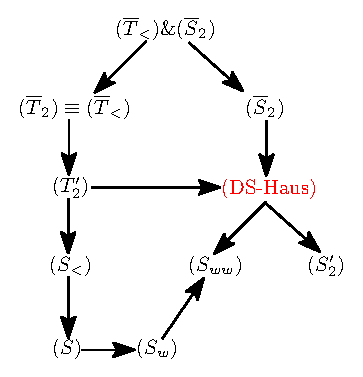
\includegraphics[width=65mm]{../img/Hausdorff_diagram.eps}
  \caption{Hausdorff type axioms}
  \label{fig:haus-diagram}
\end{figure}

\begin{prop}
  The implications $[a]-[k]$ in figure~\ref{fig:haus-diagram} hold.
\end{prop}
\begin{proof}

  [a], [b], [c], [d]:
  trivial.

  [e], [f]:
  from \ref{prop:T2'=DS-Haus+S<}.

  [g]:
  For the sake of contradiction, let $p$ be semiprime yet not prime.
  Thus, there are $x_1, x_2 \ne p$ with $x_1 \wedge x_2 = p$, which means
  $x_1\not\le x_2$ and $x_1\not\ge x_2$.
  Therefore, $x_1 \vee x_2 \not\in \{ x_1, x_2 \}$, and using weakly Hausdorff
  property, there exist $u\not\le x_1, v\not\le x_2$ with $u \wedge v = 0$.
  Hence, $u, v\not\le x_1 \wedge x_2 = p$, contradicting the semiprimeness
  of~$p$.

  [h]:
  from \ref{prop:DS-Haus->S2'}.

  [i]:
  For the sake of contradiction, consider a~semiprime~$p$ that is not a~coatom,
  that is, $p < a < 1$ for some $a$.
  By~$(S_<)$ we obtain $u\not\le a, v\not\le p$ such that $u \wedge v = 0$.
  Hence, using semiprimeness, $u \le p$ and thus $u < a$, a~contradiction.

  [j], [k]:
  from \ref{prop:S->Sw->Sww}.
\end{proof}

\section{Adding the subfitness}

Subfitness cause $(\overline{S}_2), (S_2'), (\overline{T}_2), (T_2')$ and
(DS-Haus) to coincide as it is seen from

\begin{thm}
  $(S_2')\&\text{(Sfit)}$ implies $(\overline{S}_2)\&(T_<)$.
\end{thm}

\begin{lem}
  $(S_2')\&\text{(Sfit)}$ implies (DS-Haus).
\end{lem}
\begin{proof}
  Let $a \vee b\not\in \{ a, b \}$.
  Firstly, $a\not\ge b$ means $a \ne 1$.

  Secondly, since $a\not\le b$, by subfitness we have some $c$ with $a \vee c =
  1 \ne b \vee c$.
  Thus, $a\not\le b \vee c$ (otherwise $b \vee c \ge a \vee c = 1$) and again
  $b \vee c \ne 1$.

  As also $a \vee (b \vee c) = 1$, by $(S_2')$ we get $u\not\le a$ and
  $v\not\le b \vee c$ (leading to $v\not\le b$) such that $u \wedge v = 0$.
\end{proof}

\chapter{Regularity}

\section{The $T_3$ axiom}

\begin{framed}
  \begin{df}[$T_3$]
    A~topological space~$X$ is \emph{regular\/} (or satisfies the~$T_3$
    \emph{axiom\/}) when
    \begin{center} \it
      for any $x\in X$ and any closed $A \not\owns x$ there are disjoint open
      $V_1, V_2$ such that $V_1\owns x$ and $V_2\supseteq A$.
    \end{center}
  \end{df}
\end{framed}

Even though the definition concerns points, it may be reformulated without
them.

\begin{prop} \label{topreg-char}
  A space $X$ is regular iff each $U\in \Omega(X)$ can be described as
  \[
    U = \bigcup \{V\in \Omega(X) \st \overline{V} \subseteq U\}.
  \]
\end{prop}
\begin{proof}
  The inclusion~$\supseteq$ is obvious.

  $\Rightarrow$:
  Choose an~$x\in U$.
  Since $A := X\setminus U \not\owns x$ is closed, the existence
  of~$V_1$~and~$V_2$ from $(T_3)$ is stipulated.
  The disjointedness $V_1 \cap V_2 = \none$ leads to $V_1\subseteq X\setminus
  V_2$, which is a closed set.
  Therefore, $\overline{V_1}\subseteq X\setminus V_2$.

  Furthermore, the relation $A\subseteq V_2$ is equivalent to the relation
  $X\setminus V_2\subseteq X \setminus A = U$.
  Hence, for $V_x := V_1$ one has $\overline{V_x}\subseteq X\setminus V_2\subseteq
  U$.
  Such a~system $\{V_x \st x\in U\}$ constitutes a~subset cover of $U$, and
  consequently, finishes the proof of~the~inclusion $\subseteq$.

  $\Leftarrow$:
  With $U := X\setminus A$ take $V_x$ from above and set $V_1 := V_x$ and $V_2
  := X\setminus \overline{V_x}$.
\end{proof}

Now we will deal with the~closure in the~formula:

\begin{lem} \label{lem:rb-char}
  $\overline{V}\subseteq U \quad \equiv \quad \exists W\in \Omega(X)\colon W \cap V =
  \none \;\; \& \;\; W \cup U = X$.
\end{lem}
\begin{proof}
  $\Rightarrow$:
  Take $W := X\setminus \overline{V}$.

  $\Leftarrow$:
  Recall closure's definition.
  Suppose $z\in \overline{V}\setminus U$.
  Since $W \cup U = X$, the $z$ must lie in the $W$.
  Howbeit, the $W$ does not intersect the $V$---making $z\not\in \overline{V}$.
\end{proof}

Without loss of generality, the $W$ may be replaced by~the
pseudocomplement~$V^*$ in~$\Omega(X)$, that is, by the open set $X\setminus
\overline{V}$.

\begin{rem}
Pseudocomplements always exist in frames:
setting
\[
  a^* := \bigvee \{x \st x \wedge a = 0\},
\]
we have
\[
  a^* \wedge a = \bigvee \{x \st x \wedge a = 0\} \wedge a = \bigvee \{x \wedge
  a \st x \wedge a = 0\} = 0
\]
(the second equality from the frame distributivity), and hence thus defined
$a^*$ is~the~largest $x$ such that $a \wedge x = 0$.
\end{rem}

\section{Regular locales}

\begin{framed}
  \begin{nota}[$\rb$]
    \[
      V \rb U \quad \equiv \quad V^* \vee U = 1,
    \]
    which is referred to by pronouncing \emph{``V is rather below U''\/}.
  \end{nota}
\end{framed}

\begin{lem} \label{rb->leq}
  $a \rb b \Rightarrow a \leq b$.
\end{lem}
\begin{proof}
  Using~distributivity, we have
  \[
    a = a \wedge 1 = a \wedge (a^* \vee b) = (a \wedge a^*) \vee (a \wedge b) =
    0 \vee (a \wedge b) = a \wedge b. \qedhere
  \]
\end{proof}

With $\rb$ notation we are able to adopt the characterization~\ref{topreg-char}
by~defining regularity as~follows:
\begin{framed}
  \begin{df}[Reg]
    A locale is called \emph{regular\/} if
    \[
      a = \bigvee \{x \st x \rb a\}
    \]
    for all its elements $a$.
  \end{df}
\end{framed}

Thus, we observe that
\begin{center} 
  \emph{a topological space $X$ is regular iff its $\Omega(X)$ is regular.\/}
\end{center}

\section{Strength of regularity}

\begin{lem} \label{oplus-vee-distrib}
  ~
  \begin{enumerate}
  \item $\bigvee_{i\in J} \left(a_i \oplus b\right) = \left(\bigvee_{i\in J}
    a_i \right) \oplus b$.
  \item $\bigvee_{i\in J} \left(a \oplus b_i\right) = a \oplus
    \left(\bigvee_{i\in J} b_i \right)$.
  \item $\left(\bigvee_{i\in J} a_i\right) \oplus \left(\bigvee_{j\in J}
    b_j\right) = \bigvee_{i, j\in J} \left(a_i \oplus b_j\right)$.
  \end{enumerate}
\end{lem}
\begin{proof}
  (i):
  Recall \ref{oplus-iota} on page~\pageref{oplus-iota}\thinspace.
  We have
  \begin{align*}
    \left(\bigvee_{i\in J} a_i \right) \oplus b
    &= \iota_1\left(\bigvee_{i\in J} a_i \right) \wedge \iota_2(b)
    = \left(\bigvee_{i\in J} \iota_1(a_i) \right) \wedge \iota_2(b) \\
    &= \bigvee_{i\in J} \left(\iota_1(a_i) \wedge \iota_2(b) \right)
    = \bigvee_{i\in J} \left(a_i \oplus b\right)
  \end{align*}
  as frame homomorphisms $\iota_i$ preserve suprema (for the second equality)
  and as the binary meet commutes with joins in frames (for the third
  equality).

  (ii):
  Analogously by symmetry.

  (iii):
  By consecutive application of (i) and (ii).
\end{proof}

\begin{lem}
  For a general locale $L$ and any of its saturated $U\in \left\uparrow
  d_L\right.$
  \[
    (a \wedge b, a \wedge b) \in U \qquad \Longrightarrow \qquad \forall x \rb
    a, \, y \rb b: \; (x, y) \in U
  \]
\end{lem}
\begin{proof}
  Beginning with $(x, y)\in x \oplus y$, we rewrite
  \begin{align*}
    x \oplus y &= (x \wedge (y^* \vee b)) \oplus (y \wedge (x^* \vee a)) \\
               &= (\; (x \wedge y^*) \; \vee \; (x \wedge b) \; ) \oplus (\; (y
    \wedge x^*) \; \vee \; (y \wedge a) \; )
  \end{align*}
  (using ``rather-belowness'' and distributivity, respectively).

  Proceeding with (iii) of Lemma~\ref{oplus-vee-distrib}\thinspace,
  \begin{align*}
     \ldots = \; &(\; (x \wedge y^*) \oplus (y \wedge x^*) \; ) \vee 
            (\; (x \wedge y^*) \oplus (y \wedge a) \; ) \; \vee \\
            \vee \; &(\; (x \wedge b) \oplus (y \wedge x^*) \; ) \vee
            (\; (x \wedge b) \oplus (a \wedge y) \; ) \\
     \subseteq \; &(y^*\oplus y) \vee (y^*\oplus y) \vee (x\oplus x^*) \vee (\;
            (a \wedge b)\oplus(a \wedge b) \;)
  \end{align*}
  where the upper-bound of the last member follows
  from~\ref{rb->leq}\thinspace.

  Besides, the ultimate expression is a subset of $U$:
  as $(x^*\oplus x), (y^*\oplus y)\subseteq d_L$ and $(a \wedge b)\oplus(a
  \wedge b)\subseteq U$ from the premise.
  In conclusion, $(x, y)\in x \oplus y \subseteq U$.
\end{proof}

\begin{thm}
  (Reg) implies (I-Haus).
\end{thm}
\begin{proof}
  We will show that regular locales satisfy \eqref{eq:meets-in-satur}\thinspace
  from~\ref{meets-in-satur} (see page~\pageref{meets-in-satur}).
  Let $(a \wedge b, a \wedge b) \in U$.
  By the previous lemma, we have $(x, y)\in U$ with $x \rb a$ and $y \rb b$.
  Recall the saturatedness on~page~\pageref{df:satur}\thinspace.
  Since $U$ is saturated,
  \[
    \left\{ (x, y) \st x \rb a \right\} \subseteq U
    \Longrightarrow
    \left(\bigvee \{x \st x \rb a\}, y\right)\in U,
  \]
  or equally, using regularity,
  \[
    \left(a, y\right)\in U
  \]
  for all $y \rb b$.
  Therefore, in the same way:
  $(a, b) = \left(a, \bigvee \{y \st y \rb b\}\right)\in U$.
\end{proof}

By Theorem~\ref{IHaus->DSHaus} on page~\pageref{IHaus->DSHaus}\thinspace, we
obtain
\begin{cor}
  (Reg) implies (DS-Haus).
\end{cor}

It will be useful to characterize (Reg) by a formula that resembles the subfit
definition:
\begin{lem} \label{reg-char}
  A locale is regular iff
  \[
    a \not\le b \qquad \Rightarrow \qquad \exists c: \quad a \vee c = 1 \quad
    \& \quad c^* \not\leq b
  \]
\end{lem}
\begin{proof}
  $\Rightarrow$:
  Suppose $a \not\le b$;
  using regularity, there is $x \rb a$ with $x \not\le b$ (otherwise $\bigvee
  \{x \st x \rb a\} \le b$).
  Let $c := x^*$.
  In other words, $x \rb a$ leads to $a \vee c = a \vee x^* = 1$.
  Additionally, $c^* \not\le b$:
  or~otherwise (from a~standard pseudocomplement property) $x \le x^{**} = c^*
  \le b$.

  $\Leftarrow$:
  By~\ref{rb->leq} we always have the inequality $\bigvee \{x \st x \rb a\} \le
  a$.
  Hence, for contradiction let us assume $a \not\le \bigvee \{x \st x \rb a\}$.
  Then there exists $c$ from the~premise.
  Specifically, $1 = a \vee c \le a \vee c^{**}$, which gives us $c^* \rb a$;
  and yet $c^* \not\le \bigvee \{x \st x \rb a\}$.
\end{proof}

\begin{thm} \label{thm:reg->sfit}
  (Reg) implies (Sfit).
\end{thm}
\begin{proof}
  Let $a \not\le b$.
  From Lemma~\ref{reg-char}\thinspace, we get an~element $c$ such that $a \vee
  c = 1$ and $c^* \not\le b$.
  What is more, it satisfies $b \vee c \ne 1$.
  If not so then by~distributivity
  \[
    b = b \vee 0 = b \vee (c \wedge c^*) = (b \vee c) \wedge (b \vee c^*) = 1
    \wedge (b \vee c^*) = b \vee c^*,
  \]
  which contradicts $c^* \le b$.
\end{proof}

\begin{prop} \label{prop:sloc-of-reg}
  Every sublocale $S$ of a~regular locale $L$ is also regular.
\end{prop}
\begin{proof}
  Let $h\colon L \to S$ be a~frame homomorphism.
  By~\ref{lem:rb-char}, we can formulate ``rather-belowness'' as
  \[
    a \rb b 
    \; \equiv \;
    \exists c, \; a \wedge c = 0 \text{ and } c \vee b = 1,
  \]
  Since $h(a) \wedge h(c) = h(a \wedge c) = 0$ and $h(c) \vee h(b) = h(c \vee
  b) = 1$, we have $a \rb b \Rightarrow h(a) \rb h(b)$.
  Thus, $\{ h(x) \st x \rb a\} \subseteq \{ y \st y \rb h(a)\}$, and hence,
  $
    h(a)
    = h (\bigvee \{ x \st x \rb a\})
    = \bigvee \{ h(x) \st x \rb a\}
    \le \bigvee \{ y \st y \rb h(a) \}.
  $
  The other inequality is from~\ref{rb->leq}.

  Because a~sublocale homomorphism $h$ is onto, for any $b\in S$ there is $a\in
  L$ such that
  $
    b
    = h(a)
    = \bigvee \{ y \st y \rb h(a) \}
    = \bigvee \{ y \st y \rb b \}.
  $
\end{proof}

\begin{rem}[Fitness]
  Unlike the regularity, the subfitness is not hereditary:
  in~general, not every sublocale of a~subfit locale is subfit.
  The hereditary subfitness is called \emph{fitness\/}, and by
  Proposition~\ref{prop:sloc-of-reg} and Theorem~\ref{thm:reg->sfit}, we infer
\end{rem}
\begin{obs}
  (Reg) implies the fitness.
\end{obs}

\include{chap6}
\chapter{Normality}

\section{The $T_4$ axiom}

\begin{framed}
  \begin{df}[$T_4$]
    A topological space $X$ is \emph{normal\/} (or \emph{$T_4$-space\/}) if
    \begin{center} \it
      for every disjoint closed $A, B$ there exist disjoint open $U, V$ with
      $U\supseteq A, \, V\supseteq B$.
    \end{center}
  \end{df}
\end{framed}

\section{Normal locales}

The point-free counterpart to $T_4$ is straightforward:

\begin{framed}
  \begin{df}[Norm]
    A locale $L$ is \emph{normal\/} if
    \[
      a \vee b = 1 \qquad \Rightarrow \qquad \exists u, v, \quad u \wedge v =
      0 \text{ and } a \vee u = 1 = b \vee v.
    \]
  \end{df}
\end{framed}

\begin{rem}
  As $u \wedge v = 0 \; \equiv \; v \le u^*$, we may define (Norm) equally by
  \[
    a \vee b = 1 \qquad \Rightarrow \qquad \exists u, \quad a \vee u = 1 = b
    \vee u^*.
  \]
\end{rem}

\medskip

Because the definition of $(T_4)$ is virtually point-free, we obtain following

\begin{cor}
  A topology $X$ is normal iff the locale $\Omega(X)$ is normal.
\end{cor}

\begin{lem}
  The relation $\rb$ interpolates in~normal locales.
\end{lem}
\begin{proof}
  Suppose $a$ is rather below $b$.
  That is, $a^* \vee b = 1$, and using the normality,\thinspace%
  \footnote{more precisely, the subsequent remark}
  we get $u\in L$ such that
  $a^* \vee u = 1 = b \vee u^*$.
  In other words, $a \rb u \rb b$.
\end{proof}

Combined with Remark~\ref{cb-largest-interpol} on
page~\pageref{cb-largest-interpol}\thinspace, we form

\begin{cor}
  (Norm) implies $\rb \, = \, \cb$;
  hence, in case of normal locales, regularity coincides with complete
  regularity.
\end{cor}

\begin{thm}
  (Norm) $\&$ (Sfit) $\Rightarrow$ (Reg).
\end{thm}
\begin{proof}
  Take $a\in L$ and put $b := \bigvee \{x \st x \rb a\}$.
  For contradiction, suppose that $a\not\le b$.
  Using the subfitness, there is $c\in L$ fulfilling $a \vee c = 1 \ne b \vee
  c$.
  Applying the normality, we find $u\in L$ with $a \vee u^* = 1 = c \vee u$.
  Particularly, $u \rb a$, which leads to~$u \le b$.
  Finally, $b \vee c \ge u \vee c = 1$; contradicting the subfitness.
\end{proof}

Since $\rb$ equals $\cb$ in normal locales, we also deduce

\begin{cor}
  (Norm) $\&$ (Sfit) $\Rightarrow$ (CReg).
\end{cor}

%\include{chap8}

% Ukázka použití některých konstrukcí LateXu (odkomentujte, chcete-li)
% \include{example}

\chapter*{Conclusion}
\addcontentsline{toc}{chapter}{Conclusion}

Point-free topology plays, increasingly, important role in modern mathematics
and computer science.
Therefore, it is important to know which concepts and notions of~point-set
topology have natural counterparts in~the point-free context.

In this thesis we observe that the~relationships of~$T$-axioms in~classical and
in~pointless topology are alike:
while for classical axioms it holds that
\[
  (T_4) \& (T_1)
  \; \Longrightarrow \; (T_{3\frac{1}{2}}) \& (T_1)
  \; \Longrightarrow \; (T_3) \& (T_1)
  \; \Longrightarrow \; (T_2)
  \; \Longrightarrow \; (T_1)
  \; \Longrightarrow \; (T_0),
\]
for their point-free counterparts we have
\begin{align*}
  \text{(Norm)} \& \text{(Sfit)}
  \; &\Rightarrow \; \text{(CReg)}
  \; \Rightarrow \; \text{(Reg)}
  \, \Rightarrow \; \text{(I-Haus)} \& \text{(Sfit)}
  \; \Rightarrow \\
  \; &\Rightarrow \; \text{(DS-Haus)} \& \text{(Sfit)}
  \; \Rightarrow \; \text{all axioms from chapter IV}.
\end{align*}


%%% Seznam použité literatury
%%% Seznam použité literatury je zpracován podle platných standardů. Povinnou citační
%%% normou pro bakalářskou práci je ISO 690. Jména časopisů lze uvádět zkráceně, ale jen
%%% v kodifikované podobě. Všechny použité zdroje a prameny musí být řádně citovány.

\def\bibname{Bibliography}
\begin{thebibliography}{99}
\addcontentsline{toc}{chapter}{\bibname}

%\bibitem{lamport94}
%  {\sc Lamport,} Leslie.
%  \emph{\LaTeX: A Document Preparation System}.
%  2. vydání.
%  Massachusetts: Addison Wesley, 1994.
%  ISBN 0-201-52983-1.

\bibitem{ds72}
  {\sc Dowker,} Clifford Hugh and
  {\sc Strauss,} Dona Papert.
  Separation axioms for frames.
  In: \emph{Topics in Topology}.
  1972,
  vol.~8,
  pp.~223-240.
  Proc. Colloq., Keszthely (Hungary), 1972.
  Colloq. Math. Soc. Janos Bolyai, Amsterdam: North-Holland, 1974.

\bibitem{isbell72}
  {\sc Isbell,} John Rolfe.
  Atomless parts of spaces.
  In: \emph{Mathematica Scandinavica}.
  1972,
  31:5-32.

\bibitem{picado-pultr12}
  {\sc Picado,} Jorge and
  {\sc Pultr,} Aleš.
  \emph{Frames and Locales: Topology without points}.
  2012 edition.
  Basel: Birkh\"{a}user, 2012.
  ISBN 978-3-0348-0153-9.

\end{thebibliography}


%%% Tabulky v bakalářské práci, existují-li.
%\chapwithtoc{List of Tables}

%%% Použité zkratky v bakalářské práci, existují-li, včetně jejich vysvětlení.
%\chapwithtoc{List of Abbreviations}

%%% Přílohy k bakalářské práci, existují-li (různé dodatky jako výpisy programů,
%%% diagramy apod.). Každá příloha musí být alespoň jednou odkazována z vlastního
%%% textu práce. Přílohy se číslují.
%\chapwithtoc{Attachments}

%%% Seznam obrázků
%\cleardoublepage
%\phantomsection
%\addcontentsline{toc}{chapter}{List of Figures}
%\listoffigures

\openright
\end{document}
